\setlength{\parskip}{\baselineskip} 
%\section{PCP}

\frame{\frametitle{Simulations}
\vspace{2ex}
\begin{columns}
\column{0.5\textwidth}
\begin{itemize}
	\item Matrix size
	\begin{itemize}
		\item 500 $\times$ 16
		\end{itemize}
	\item Low rank structure
	\begin{itemize}
		\item Rank: 4
		\end{itemize}
	\item Added noise
	\begin{itemize}
		\item Low \& high
		\item Added sparse events
		\end{itemize}
	\item Values $<$ LOD
	\begin{itemize}
		\item 25\%, 50\%, 75\%
		\end{itemize}
	\item Compared with PCA
       	\end{itemize}

\column{0.5\textwidth}
\vspace{2em}
\begin{center}
      %\only<1>{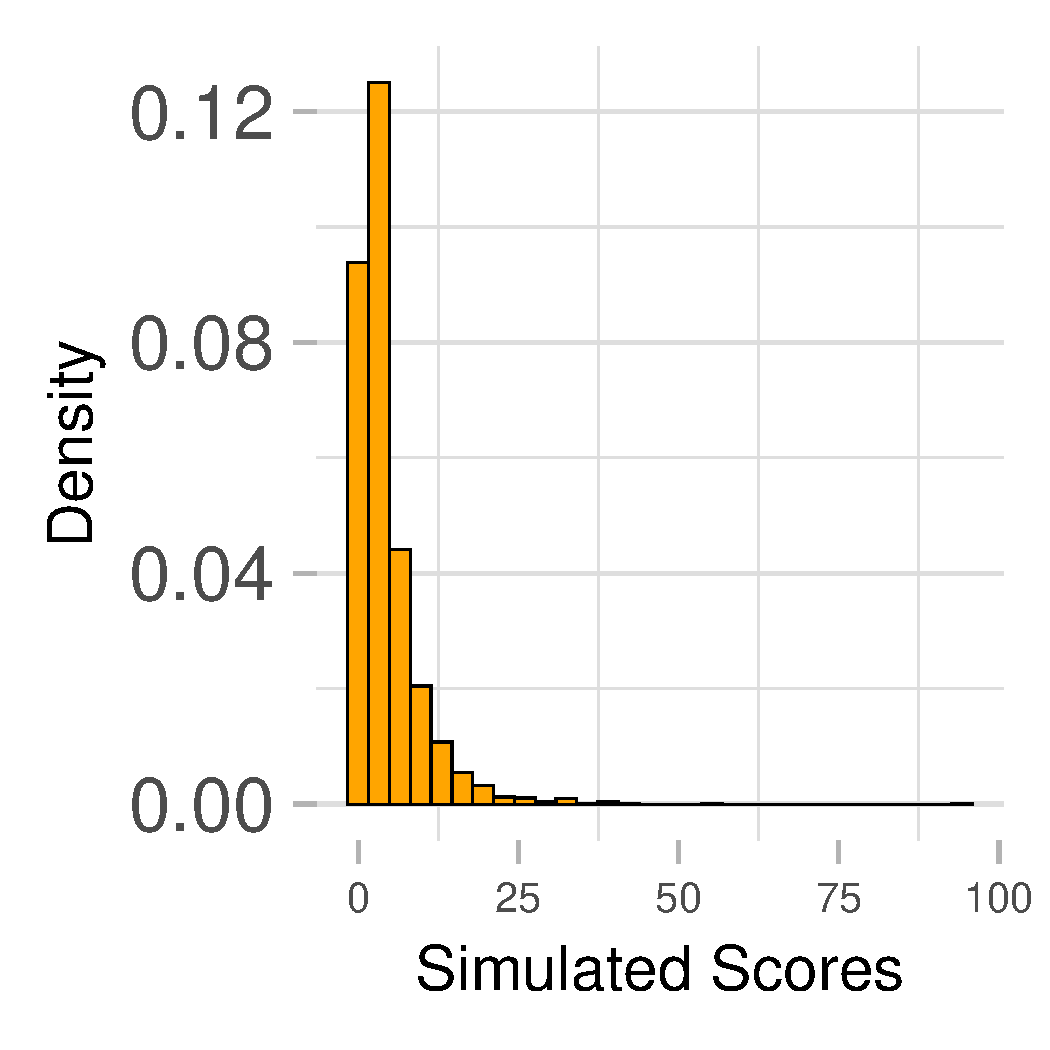
\includegraphics[height=5cm]{figures/pcp/scores_plot.pdf}}
      \only<1>{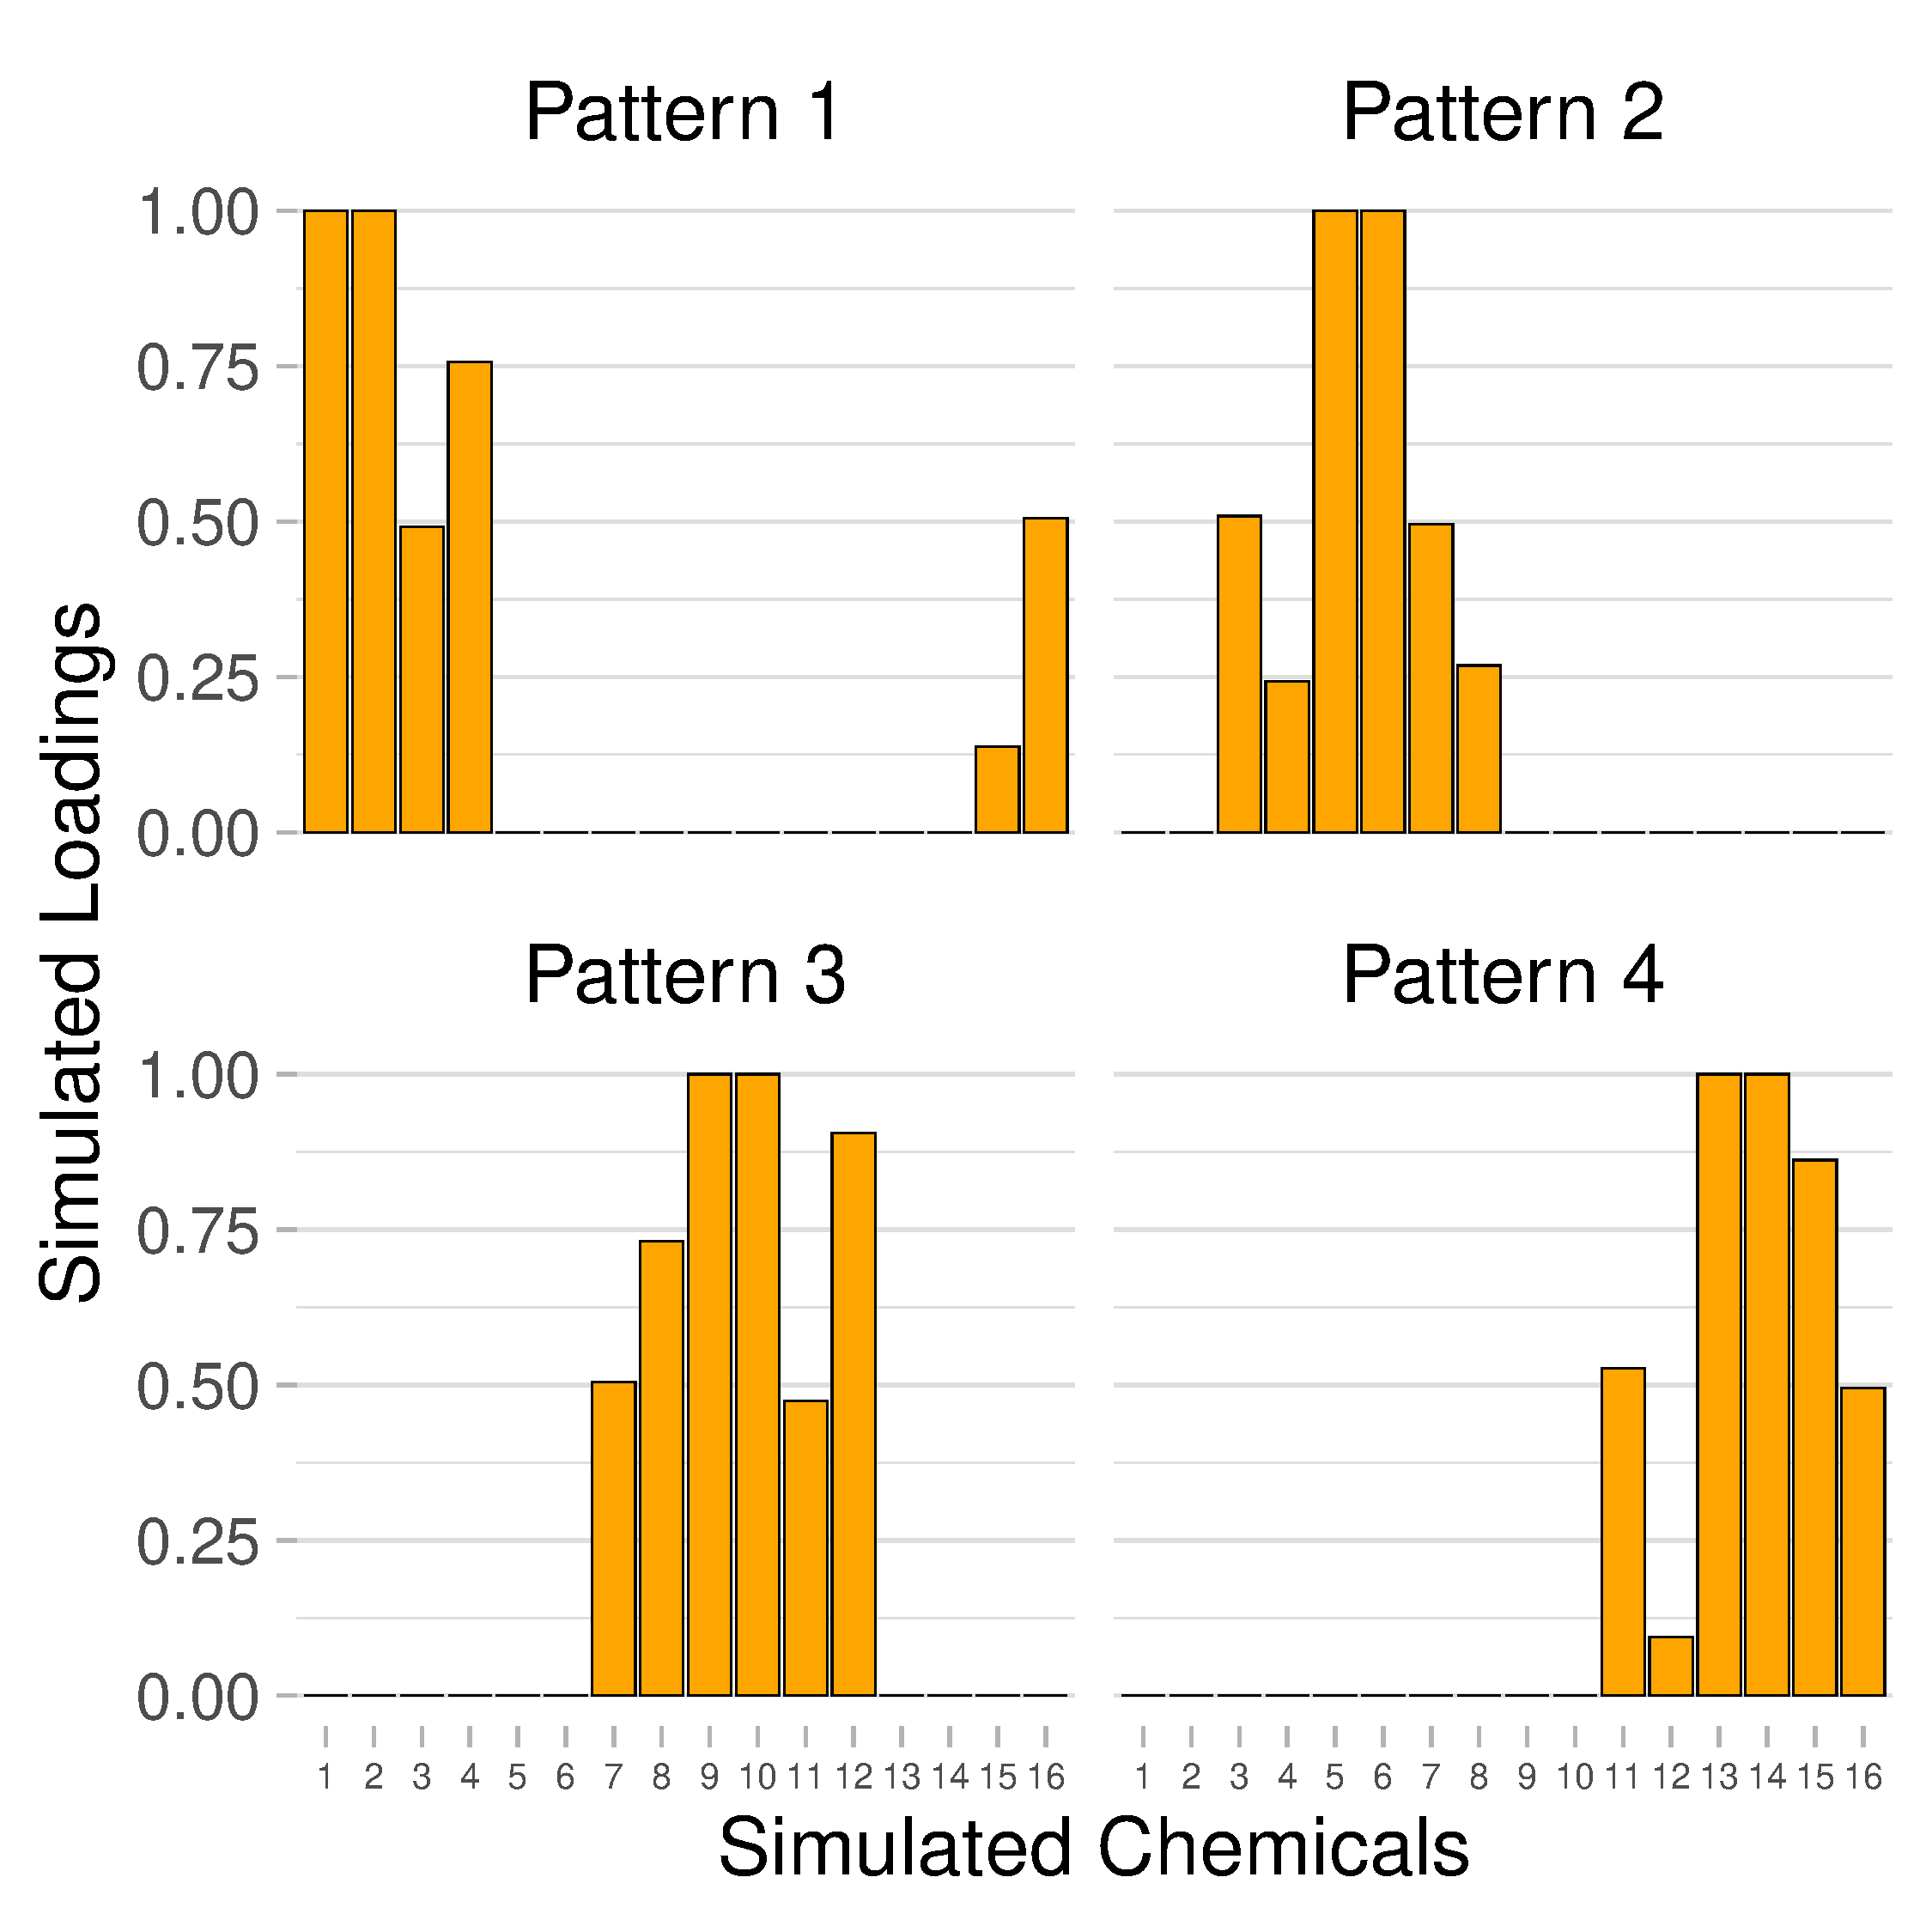
\includegraphics[height=5cm]{figures/pcp/loadings_plot.pdf}}
      %\only<2>{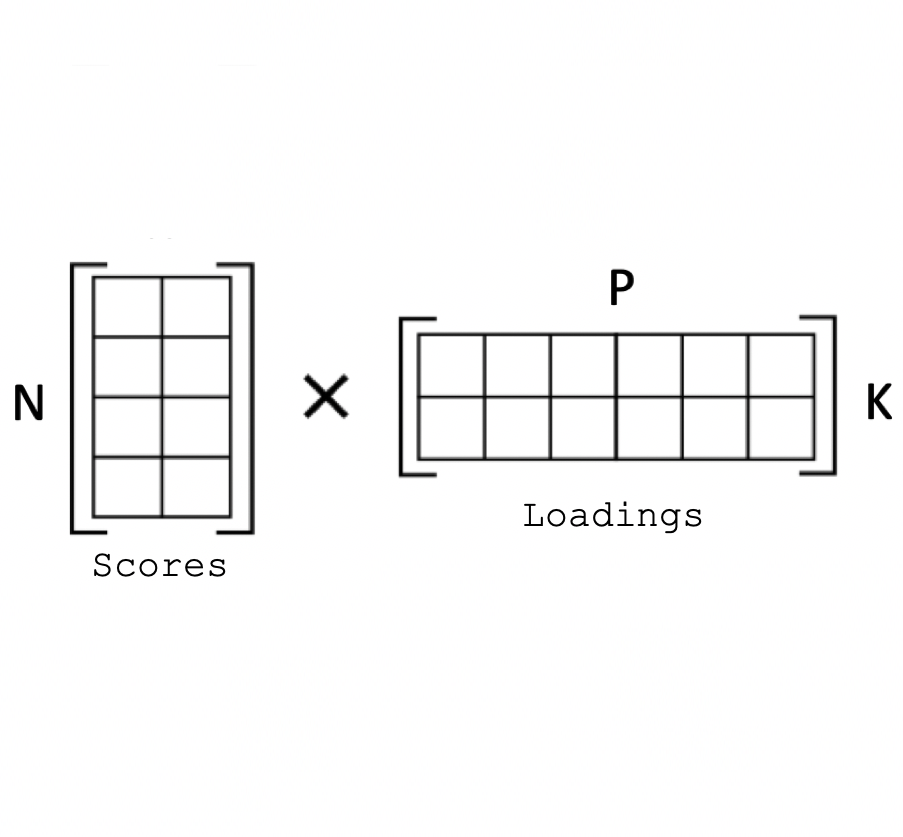
\includegraphics[height=5cm]{figures/patscore2.png}}
      \only<2>{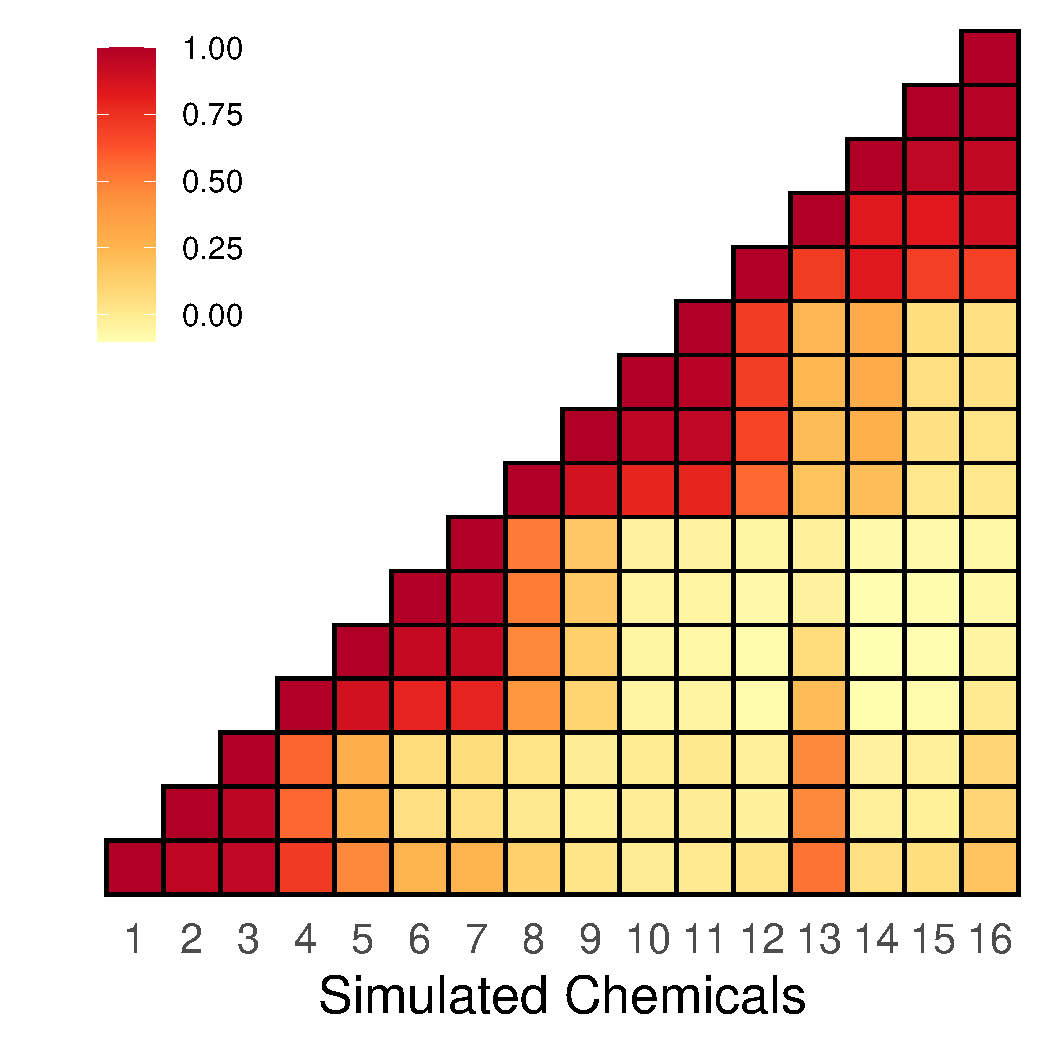
\includegraphics[height=5cm]{figures/pcp/sim_corr_pcp.pdf}}
\end{center}
\end{columns}
}

\frame{\frametitle{Simulation results: Relative error overall}
\vspace{-1ex}
\begin{center}
	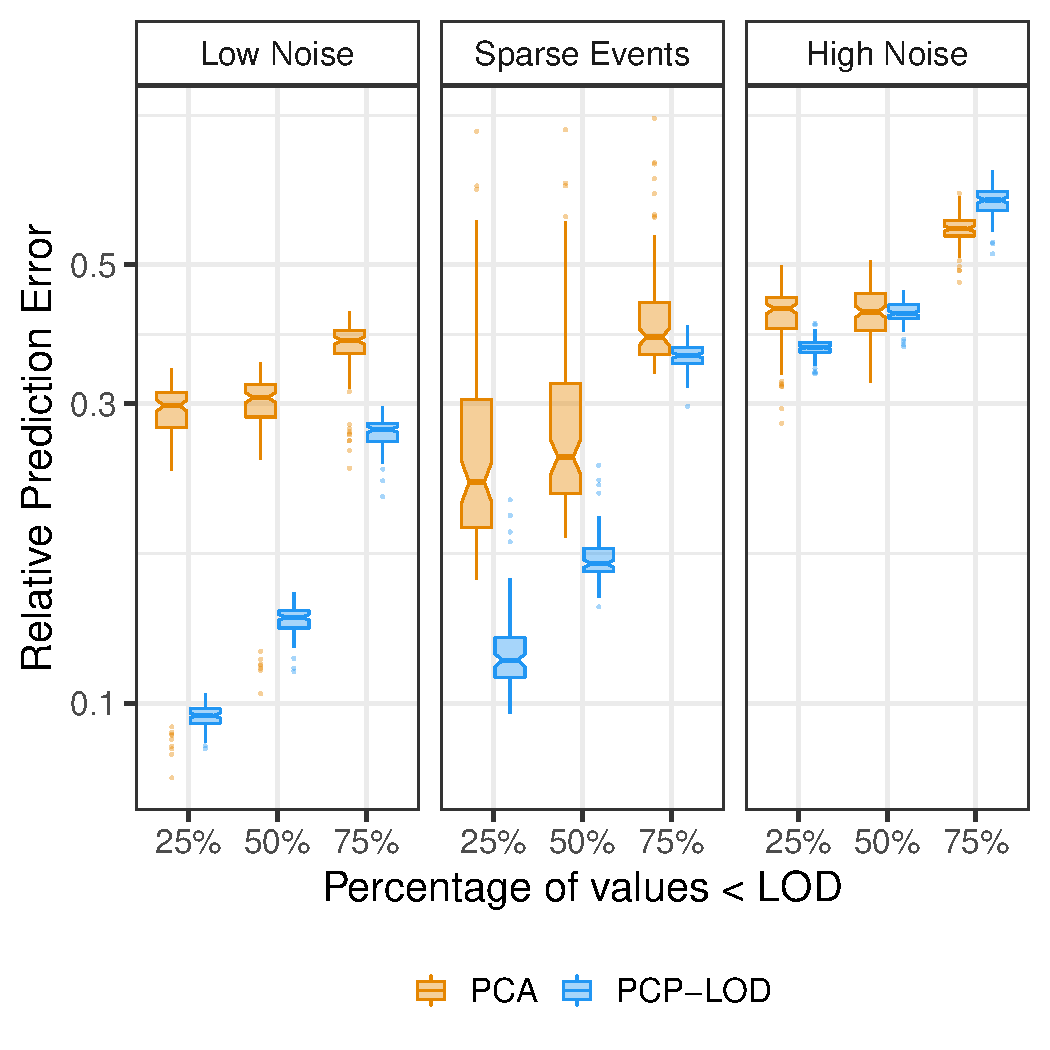
\includegraphics[scale=0.42]{figures/pcp/sim_boxplots_16.pdf}
\end{center}
}

\frame{\frametitle{Simulation results: Relative error by LOD}
\vspace{-1.25ex}
\begin{center}
	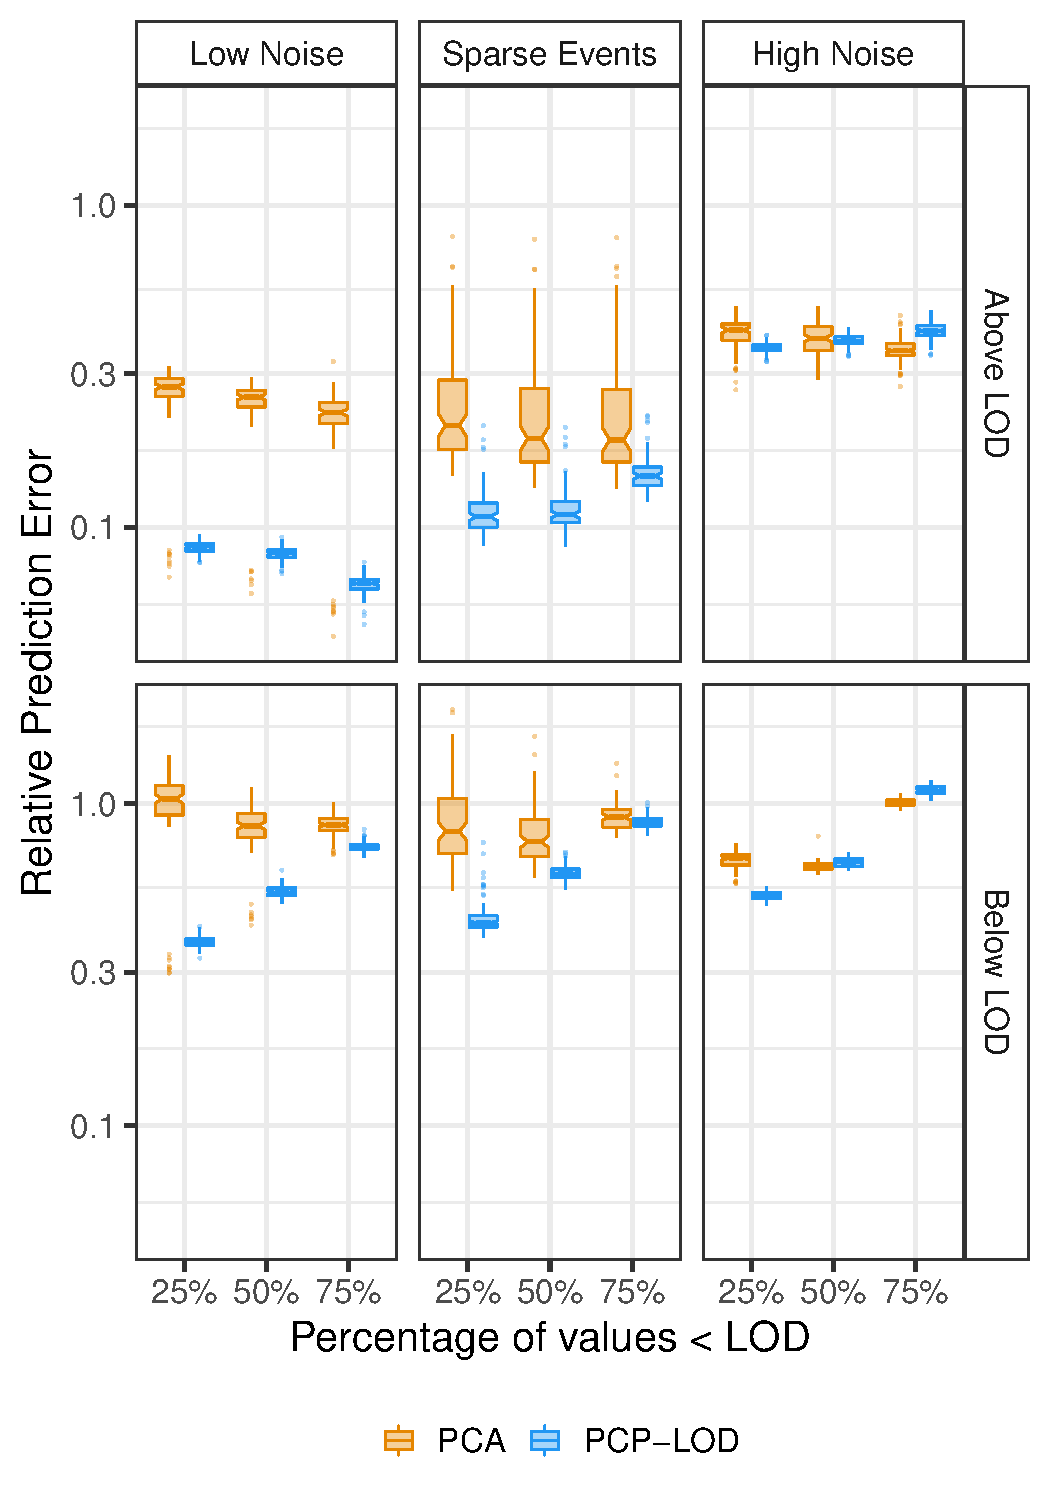
\includegraphics[scale=0.29]{figures/pcp/lod_boxplots_16.pdf}
\end{center}
}

% \frame{\frametitle{Simulation results: Relative error on loadings \& scores}
% \vspace{-1.25ex}
% \begin{center}
% 	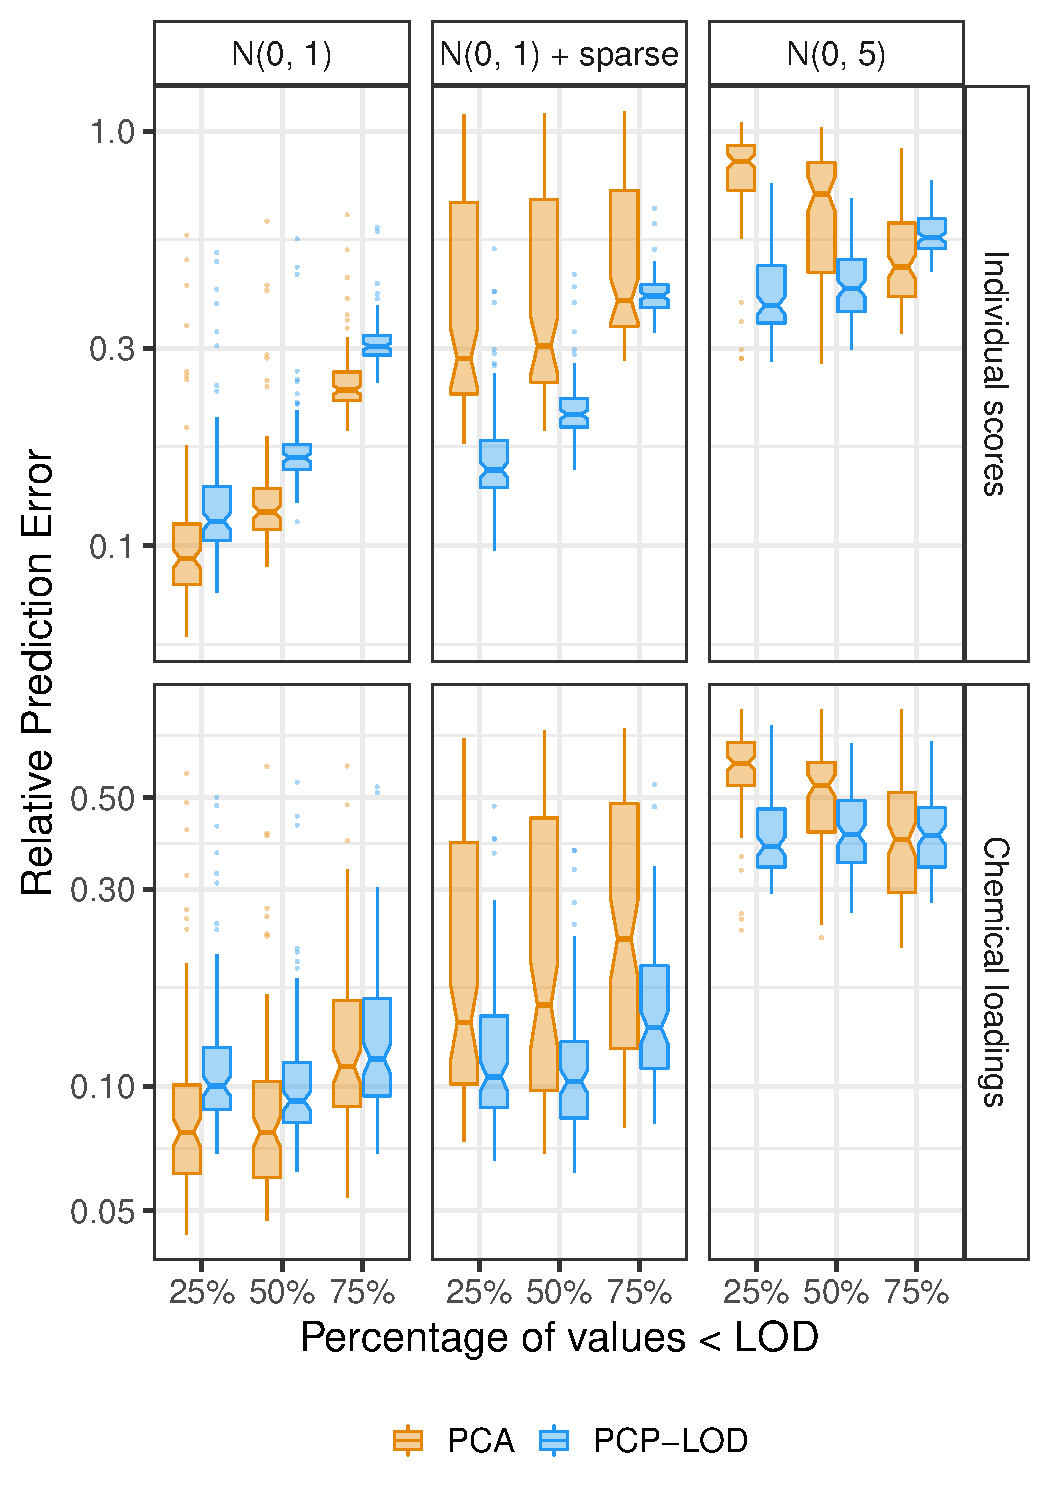
\includegraphics[scale=0.29]{figures/pcp/svd_boxplots_16.pdf}
% \end{center}
% }